\documentclass[12pt,a4paper]{book}
\usepackage[utf8]{inputenc}
\usepackage{graphicx}
\usepackage{tabularx}
\usepackage{siunitx}
\usepackage{amsmath,stix,bm}
%% fur amsmath, comment garamond and add
%% 'stix' btwn amsmath and bm
\usepackage{eucal}
%\usepackage{amsfonts}
%\usepackage{amssymb}
%\usepackage{wasysym}
%\usepackage{booktabs}
\usepackage{caption}
%\usepackage{lmodern}
\usepackage{multicol}
\usepackage[margin=0.75in,bottom=0.5in]{geometry}
%%\usepackage{avant}
%Per grafica vettoriale tramite InkScape%
\usepackage{color}
\usepackage{transparent}
\graphicspath{{img/}}
\usepackage[dvipsnames]{xcolor}
\usepackage{pdfpages}
\usepackage{pgfplots}
\usepackage{textcomp}
\usepackage{tgbonum}
\usepackage{xcolor,colortbl}
\usepackage{simpsons}
\usepackage{addfont}
\addfont[1.5]{OT1}{simfon}{\simfon}
\usepackage{listings}
%% 
\graphicspath{{figures/}} %Setting the graphicspat%h
\graphicspath{{figures/}} %Setting the graphicspath
\makeatletter
\providecommand*{\input@path}{}
\edef\input@path{{figures/}{}\input@path}% prepend
\makeatother
\usepackage{subcaption}
\begin{document}
	{\fontfamily{lmss}\selectfont

\section*{\fontfamily{qag}\selectfont\color{Turquoise}Array of folded patches}
{\color{gray}\begin{center}{\small Wireless Electromagnetic Technologies - University of Rome Tor Vergata}\end{center}}
\begin{flushright}
{\small{{\color{Mahogany}Professor:} {\color{Turquoise} Marrocco Gaetano, }}}{\small{\color{Mahogany}Students: }}{\small{\color{Turquoise}Blasi Luca, }}{\small{\color{Turquoise}Mastrofini Alessandro, }}{\small{\color{Turquoise}Mucenica Stefan Leonard}}
\end{flushright}
\subsection*{\fontfamily{qag}\selectfont\color{Turquoise}Tchebyshev array factor design}
The design of the Tchebyshev array factor will be made with five elements and a lobe/side lobe ratio of \textbf{\color{Mahogany}R\,=\,41.58\,dB}. In order to minimize the beamwidth, let's look for the optimal inter-spacing:
\begin{equation}
d_{\max}\,=\,\lambda\,\left[1-\frac{1}{2\pi}\,\arccos\left(\frac{3\,-\,x_1}{1\,+\,x_1}\right)\right]\quad \text{with}\quad d_{\max}\,\in\,\left[\frac{\lambda}{2}\,,\,\lambda\right]
\end{equation}
\begin{center}
\begin{tabular}{||c|c||}
\hline
\textbf{\color{Mahogany}Parameter}

& \textbf{\color{Mahogany}Value} \\
\hline
\textbf{Feed coefficients} $[A]$ &  \footnotesize{$\begin{bmatrix}
C_{-2}\\
C_{-1}\\
C_0\\
C_1\\
C_2\\
\end{bmatrix}\,=\,\begin{bmatrix}
9.6\\
29.8\\
41.2\\
29.8\\
9.6\\
\end{bmatrix}$}\\
\hline 
\textbf{Tapering efficiency} & \footnotesize{$\eta_T\,=\,79\,\%$}\\ 
\hline 
\textbf{Beamwidth} & $ \begin{matrix}
\text{Tchebyshev} & || & \text{Uniform} \\

50.6^\circ & || & 34.8^\circ\\
\end{matrix} $ \\
\hline 
\end{tabular}
\end{center}

\begin{center}
\begin{figure}[h]
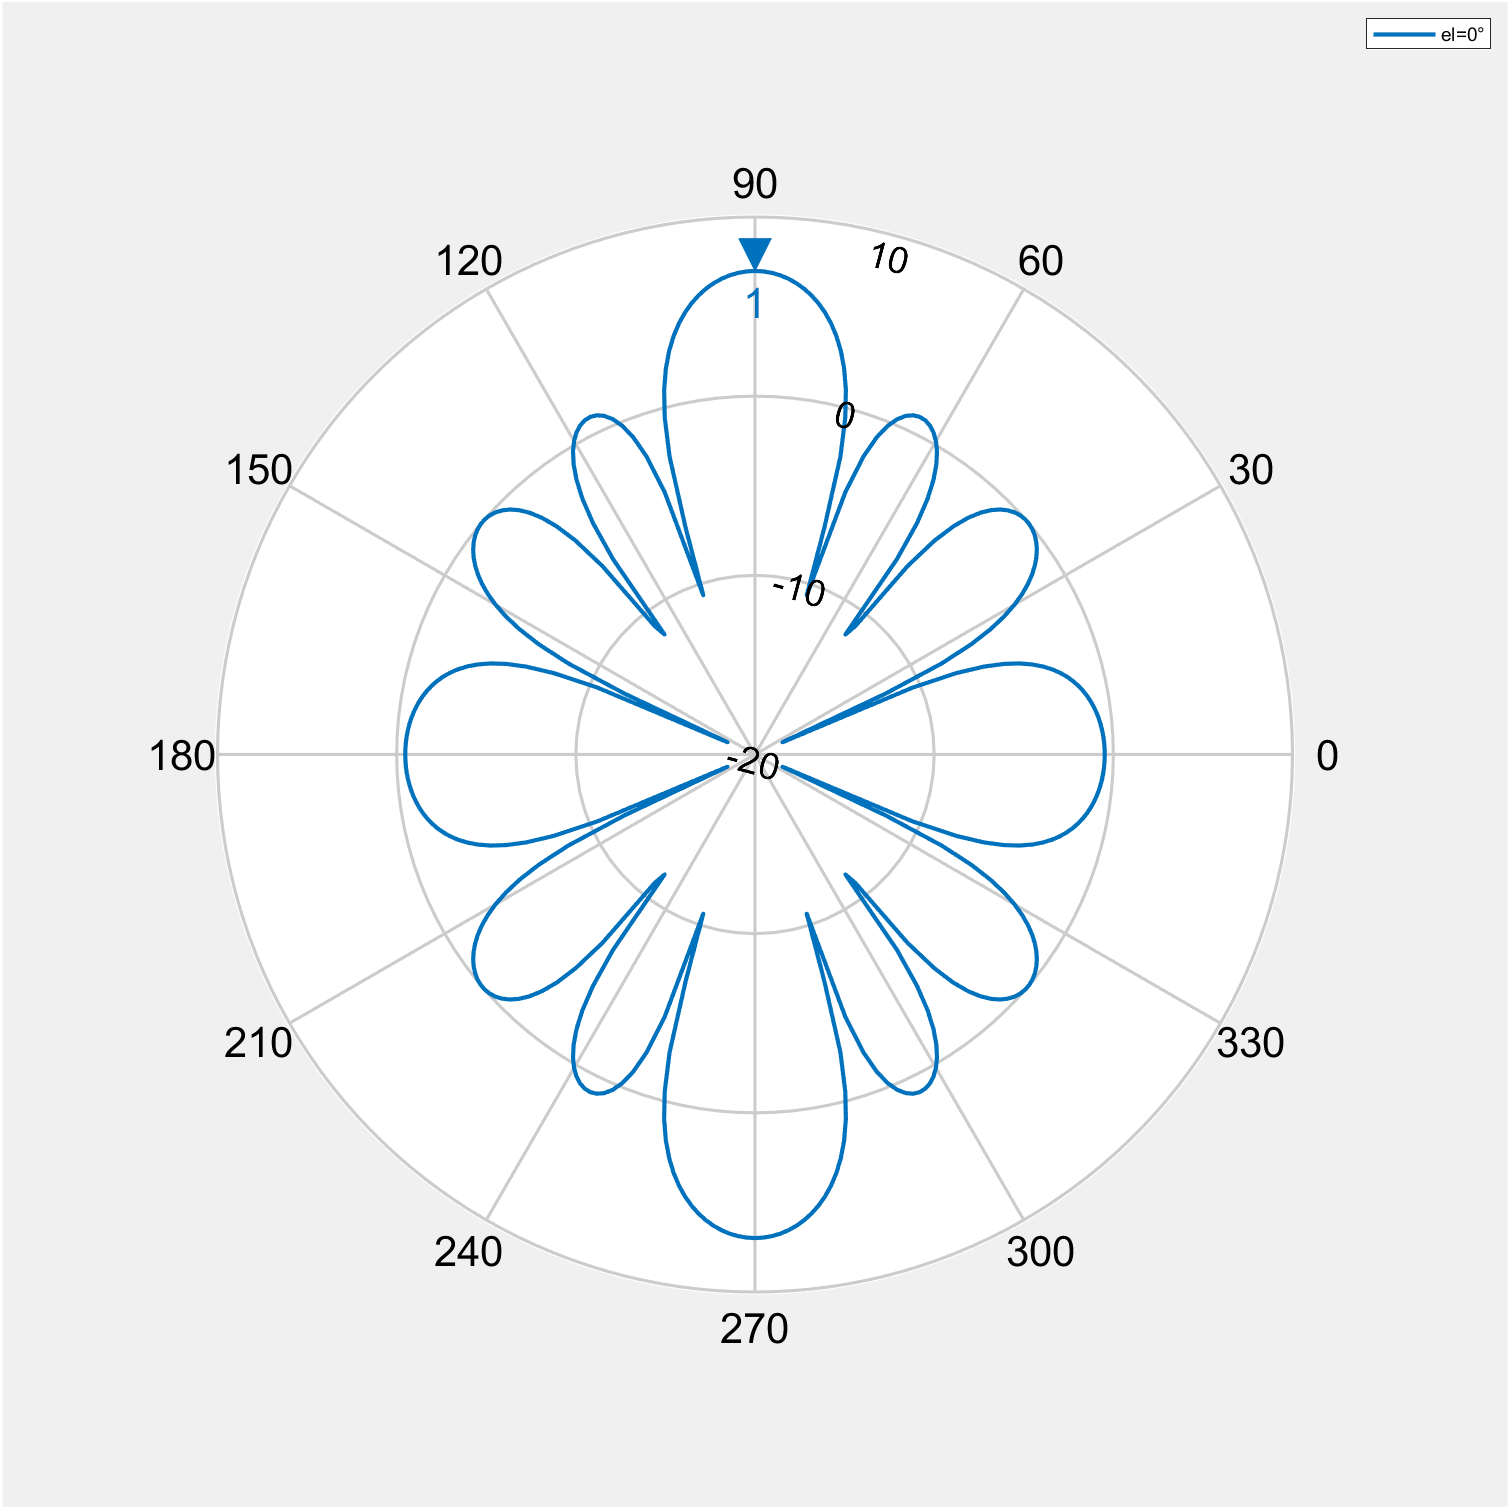
\includegraphics[scale=0.3]{array_factor_polar.png}
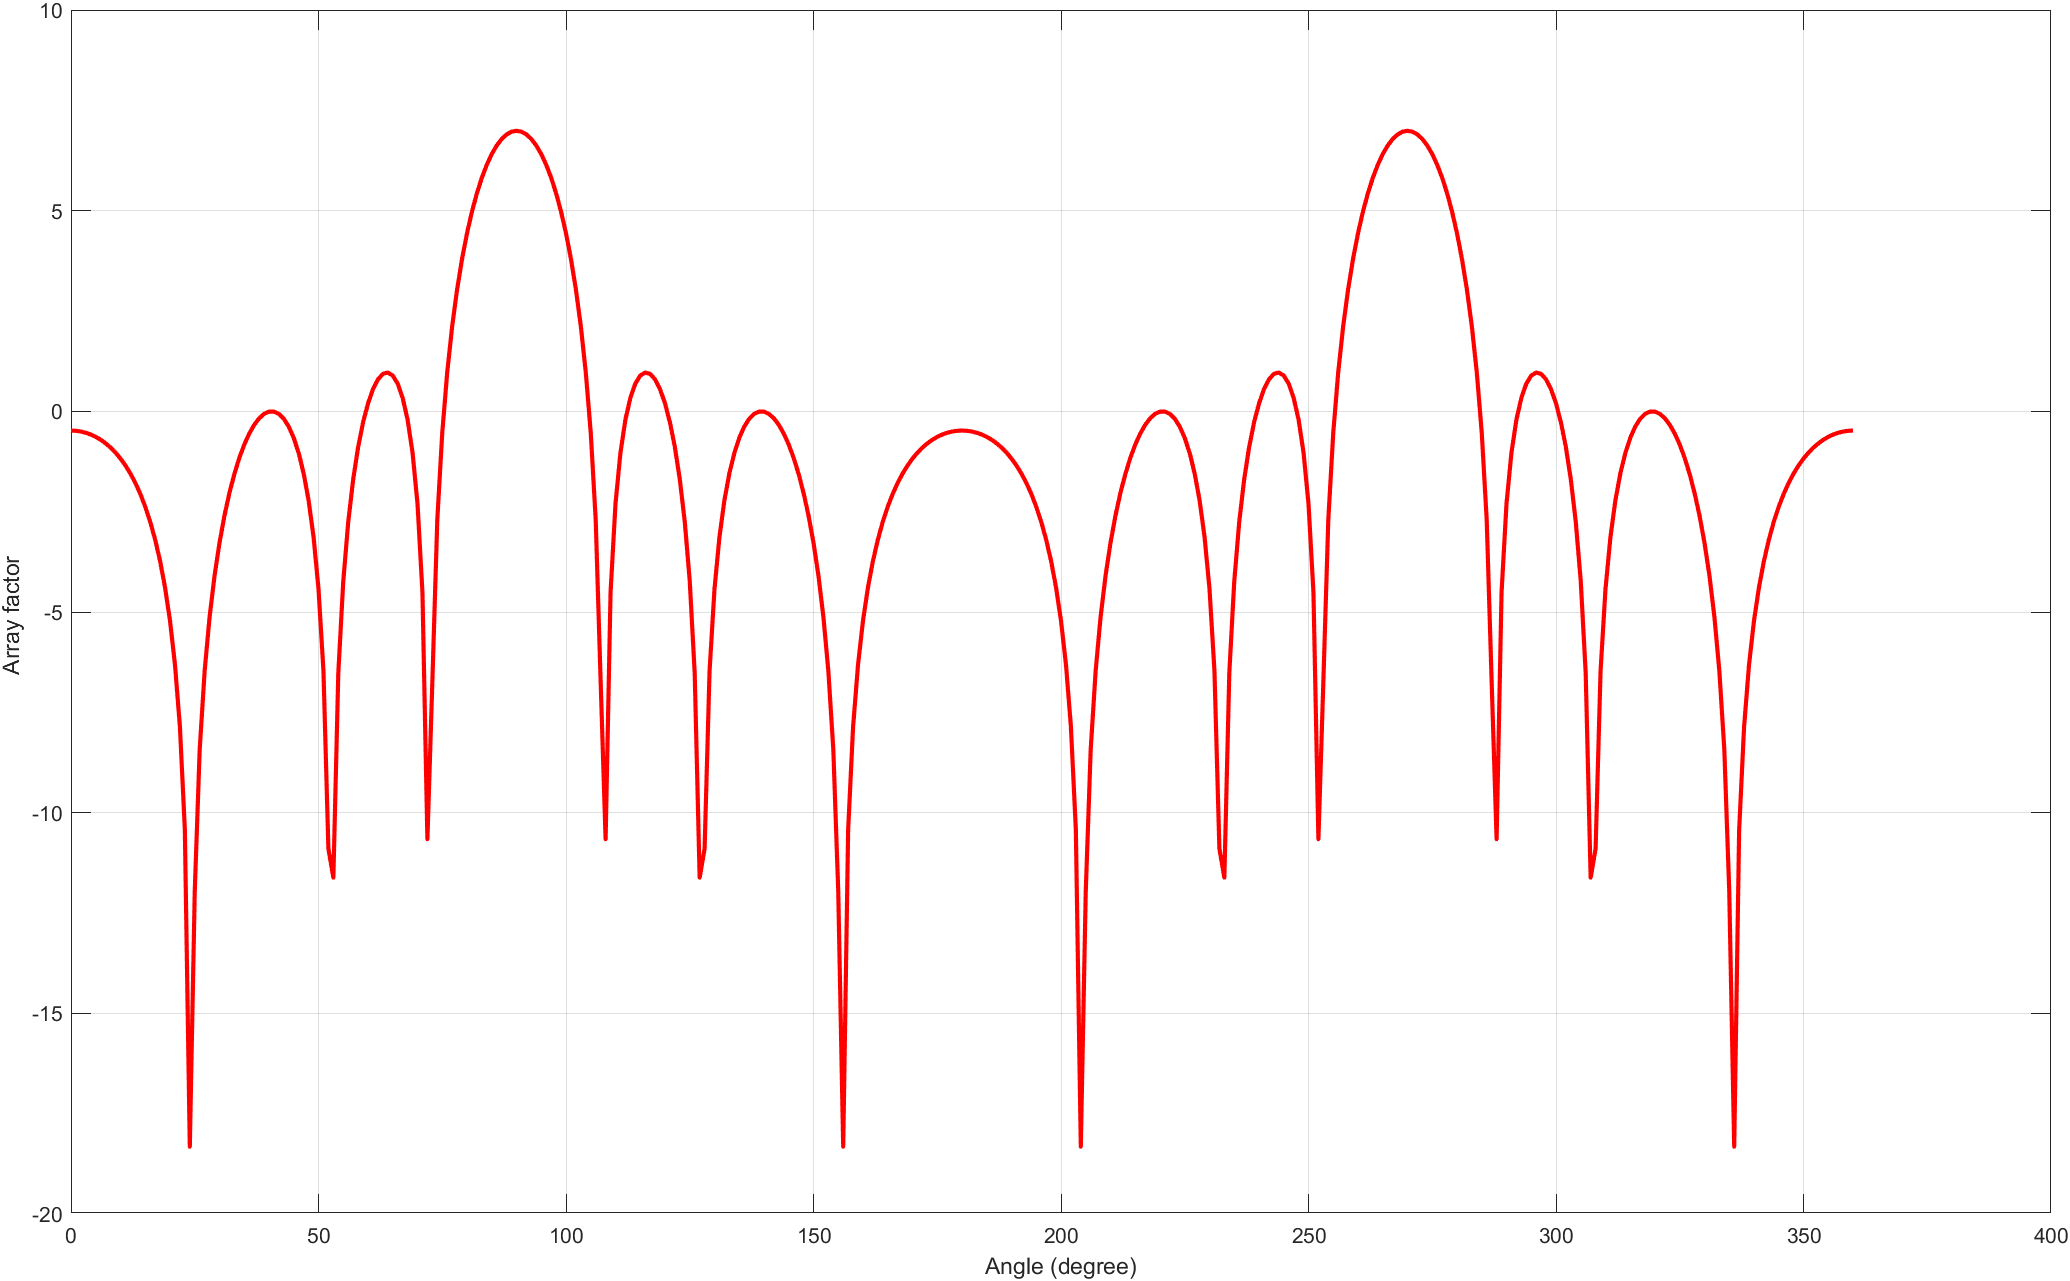
\includegraphics[scale=0.3]{array_factor_rectangular.png}
\captionof{figure}{{\color{gray}\fontfamily{lmss}\selectfont Array factor polar (left) and rectangular (right) diagrams}}
\end{figure}
\end{center}

\subsection*{\fontfamily{qag}\selectfont\color{Turquoise}Rectangular folded patch design}
\subsubsection*{\fontfamily{qag}\selectfont\color{Turquoise}Mesh density refinement}
A FR4 substrate thickness of $h_{sub}\,=\,0.8\,mm$  has been selected so it could be considered as a thin one:
\[\lambda_{sub}\,=\,0.0652\,m\quad \leadsto\quad \frac{h_{sub}}{\lambda_{sub}}\,\cong\,\frac{1}{81}\]
In case of thin substrates ($h/\lambda\,\leq\,1/50$),  the \texttt{\color{Mahogany}Antenna Toolbox} suggests to mesh the antenna using dielectric in auto mode. The other two available substrate thicknesses ($1.0\,mm$ and $1.6\,mm$) have not been adopted because the \texttt{\color{Mahogany}Antenna Toolbox} reference doesn't give any information about accuracy of the results in case of $h_{sub}\,\in\,\left(\frac{\lambda}{50}\,,\,\frac{\lambda}{10}\right)$. 
\begin{center}
\begin{figure}[h]
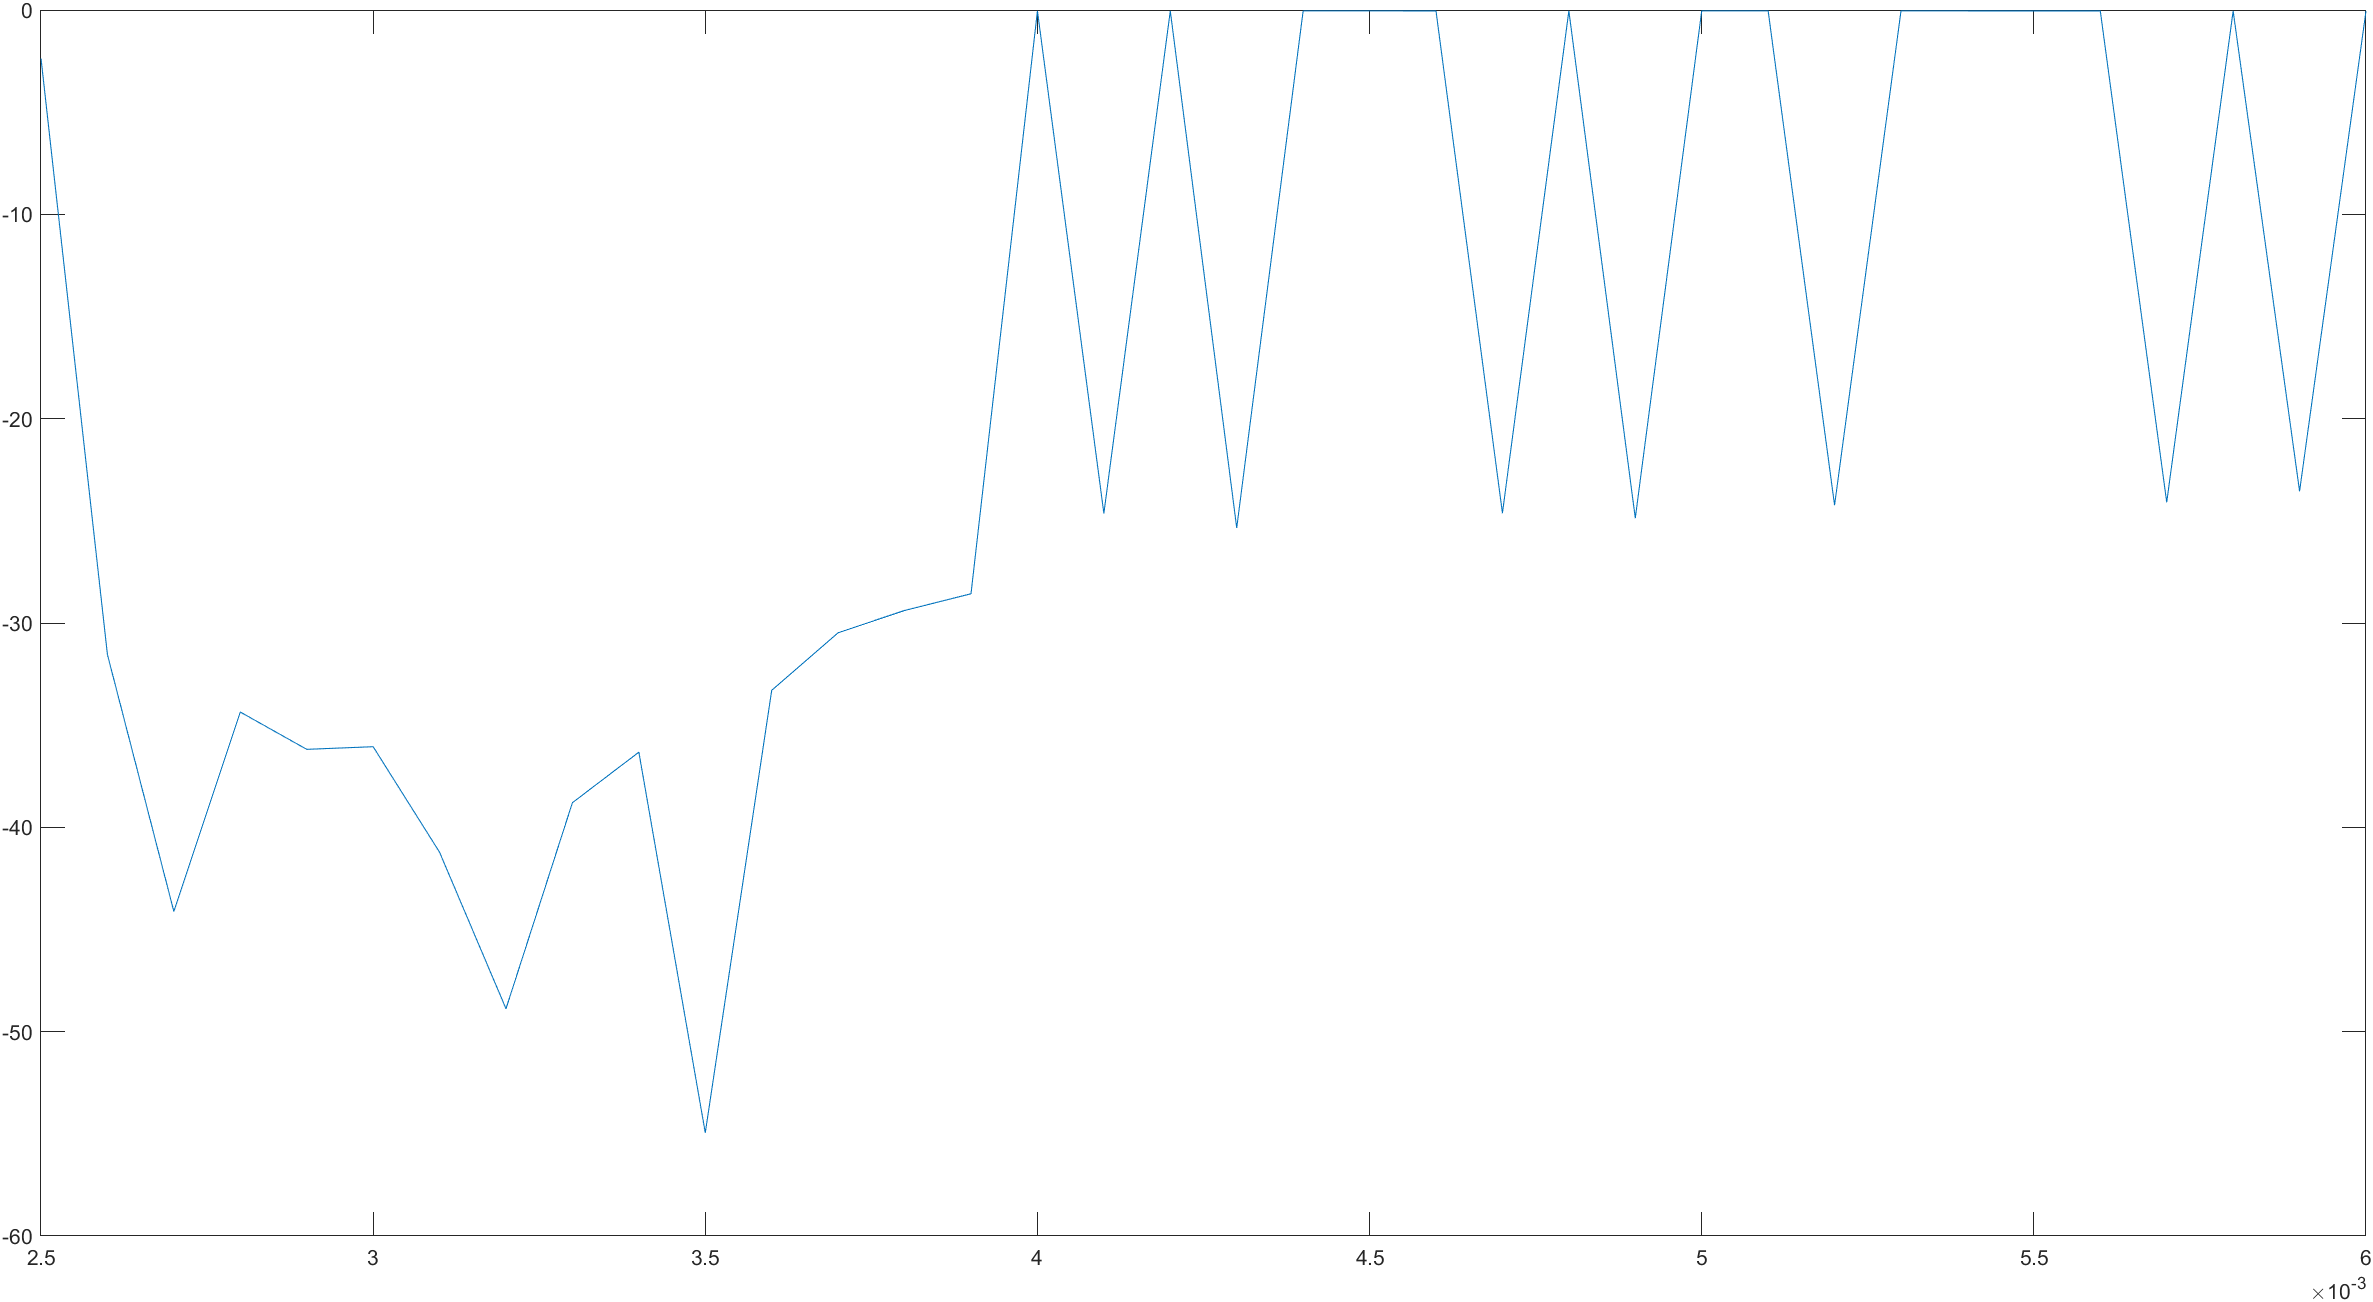
\includegraphics[scale=0.3]{mesh_levels.png}
\captionof{figure}{{\color{gray}\fontfamily{lmss}\selectfont Minimum of the reflection coefficient $\Gamma\, [dB]$ in the frequency range $2.0\div 2.2\,GHz$ depending on the varying mesh density level}}
\end{figure}
\end{center}
\subsubsection*{\fontfamily{qag}\selectfont\color{Turquoise}Patch parameters}
\begin{equation}\begin{aligned}L\,+\,W\,-\,w_{SC}\,&{\color{Mahogany}=}\,\frac{\lambda}{4}\,+\,h_{sub}\\
W\,&{\color{Mahogany}=}\,\frac{\lambda_0}{2}\,\sqrt{\frac{2}{\varepsilon_r\,+\,1}}\\
\end{aligned}
\end{equation}
\begin{equation}
\begin{aligned}
BW_E\,&{\color{Mahogany}=}\,2\,\arccos\,\sqrt{\frac{7.03\,\lambda_0^2}{4\,(3\,L_e^2+h^2)\,\pi^2}}\\
BW_H\,&{\color{Mahogany}=}\,2\,\arccos\sqrt{\frac{1}{2\,+\,k_0\,W}}\\
\end{aligned}
\end{equation}
\begin{equation}
\ell_{feed}\,{\color{Mahogany}=}\,\frac{L}{\pi}\,\arccos\,\sqrt{\frac{R_{in}}{R_r}}
\end{equation}
%% w_{feed} = 0.001 

\begin{center}
\begin{figure}
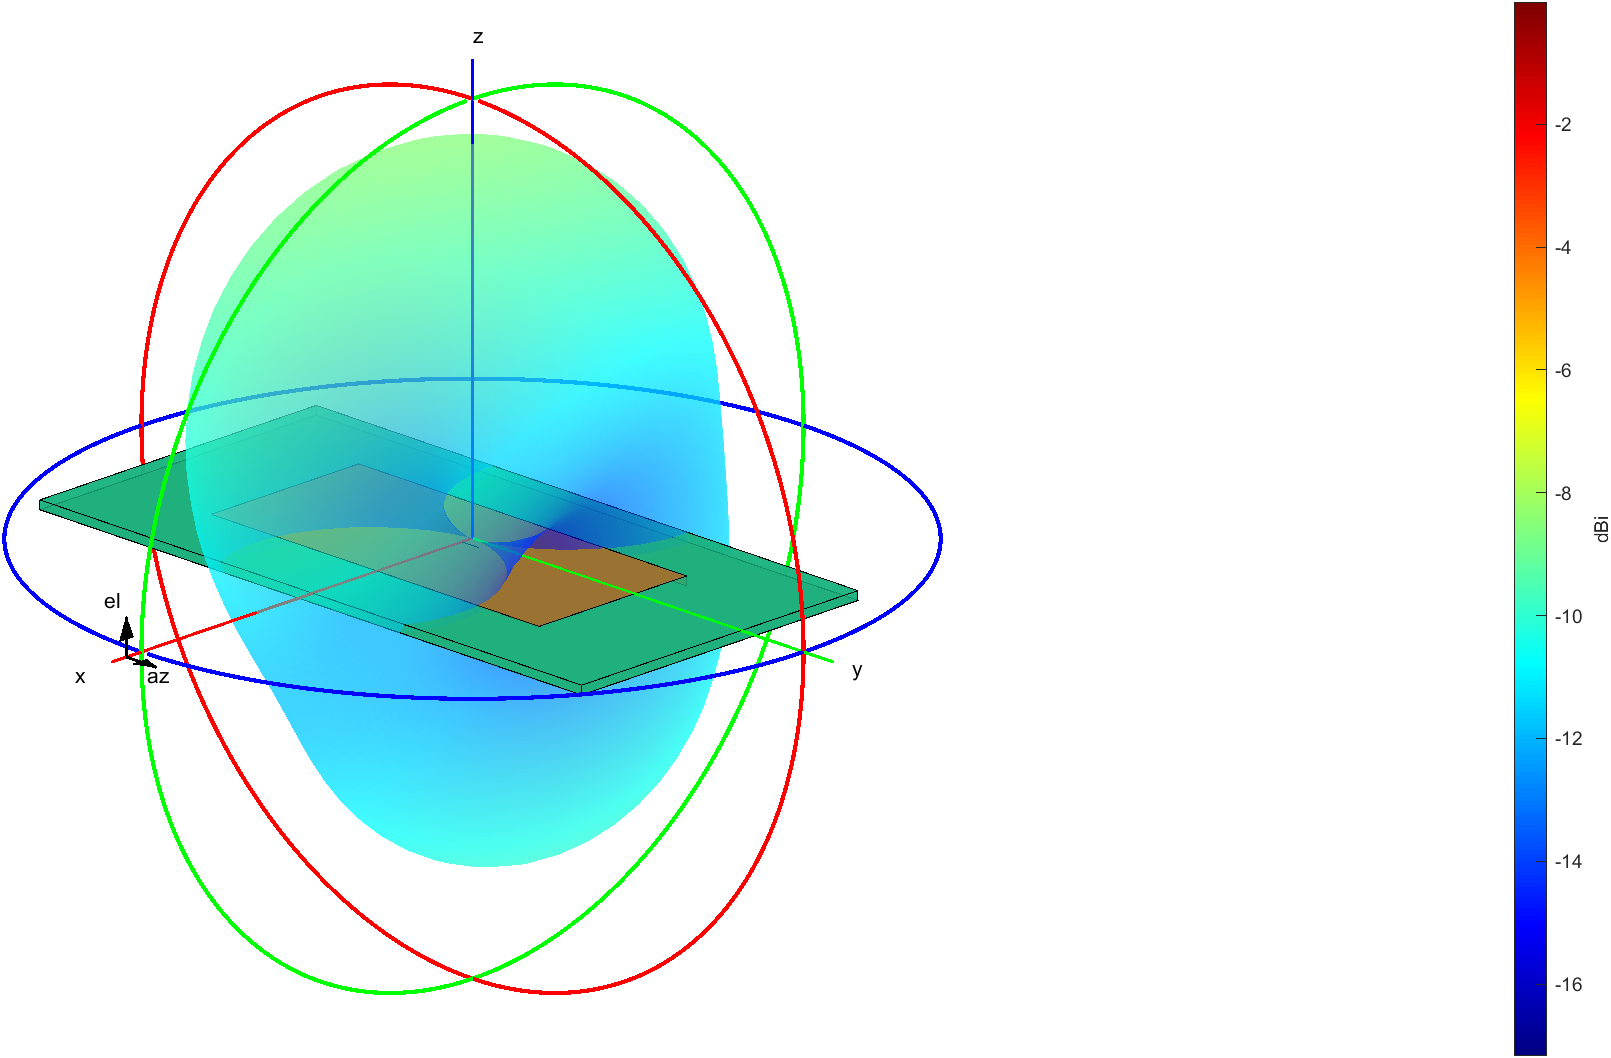
\includegraphics[width = 0.3\linewidth]{gain_patch.png}
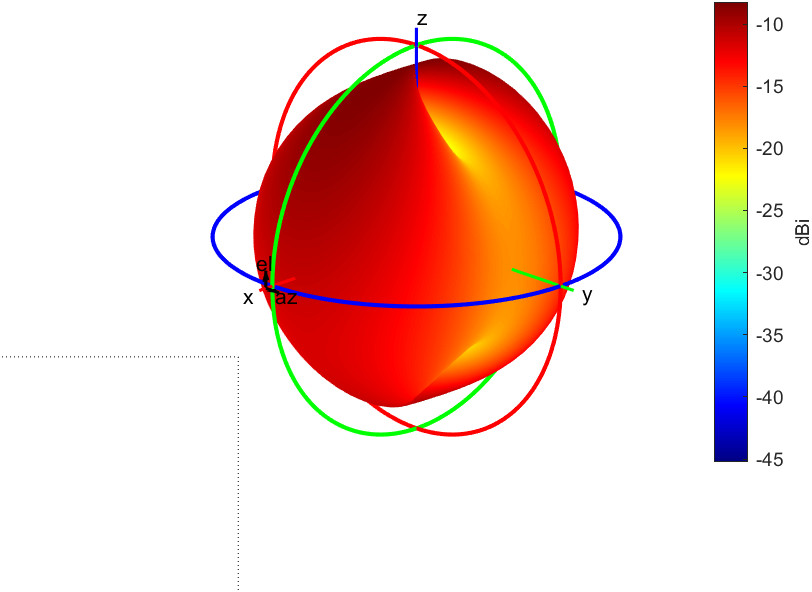
\includegraphics[width = 0.3\linewidth]{gain_patch_v.png}
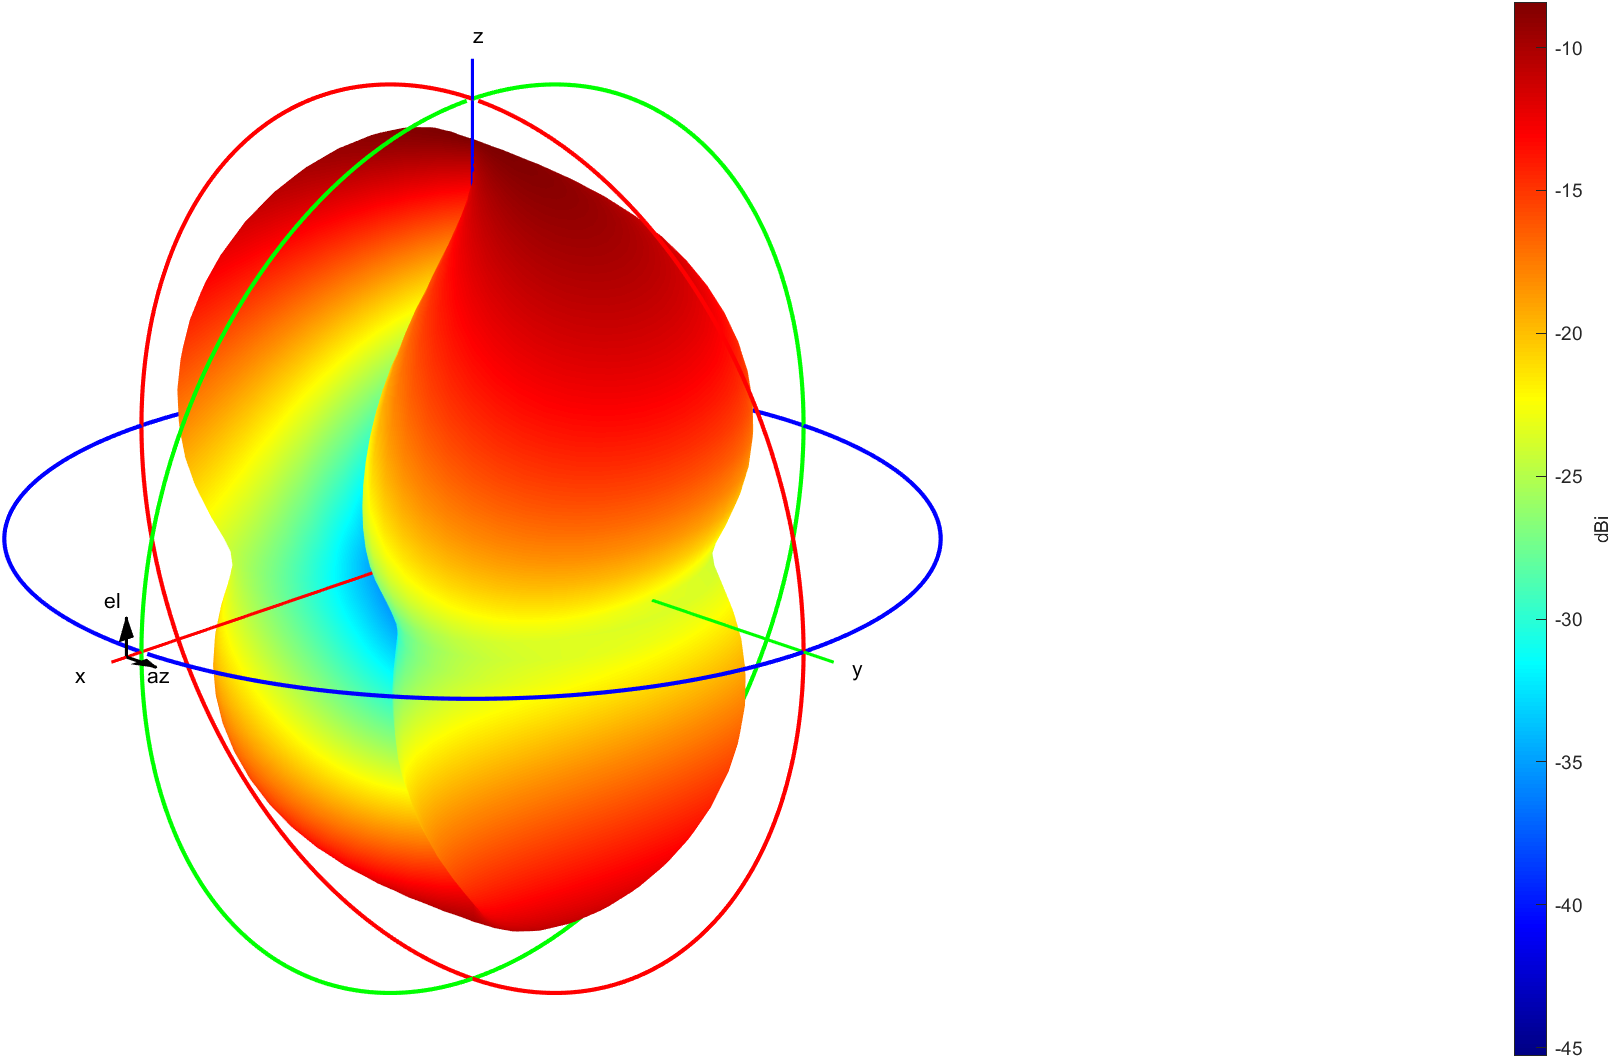
\includegraphics[width = 0.3\linewidth]{gain_patch_h.png}
\captionof{figure}{\color{gray}\fontfamily{lmss}\selectfont Gain pattern (left), gain pattern with vertical polarization (center) and with the horizontal one (right)}
\end{figure}
\end{center}
\begin{center}
\begin{figure}
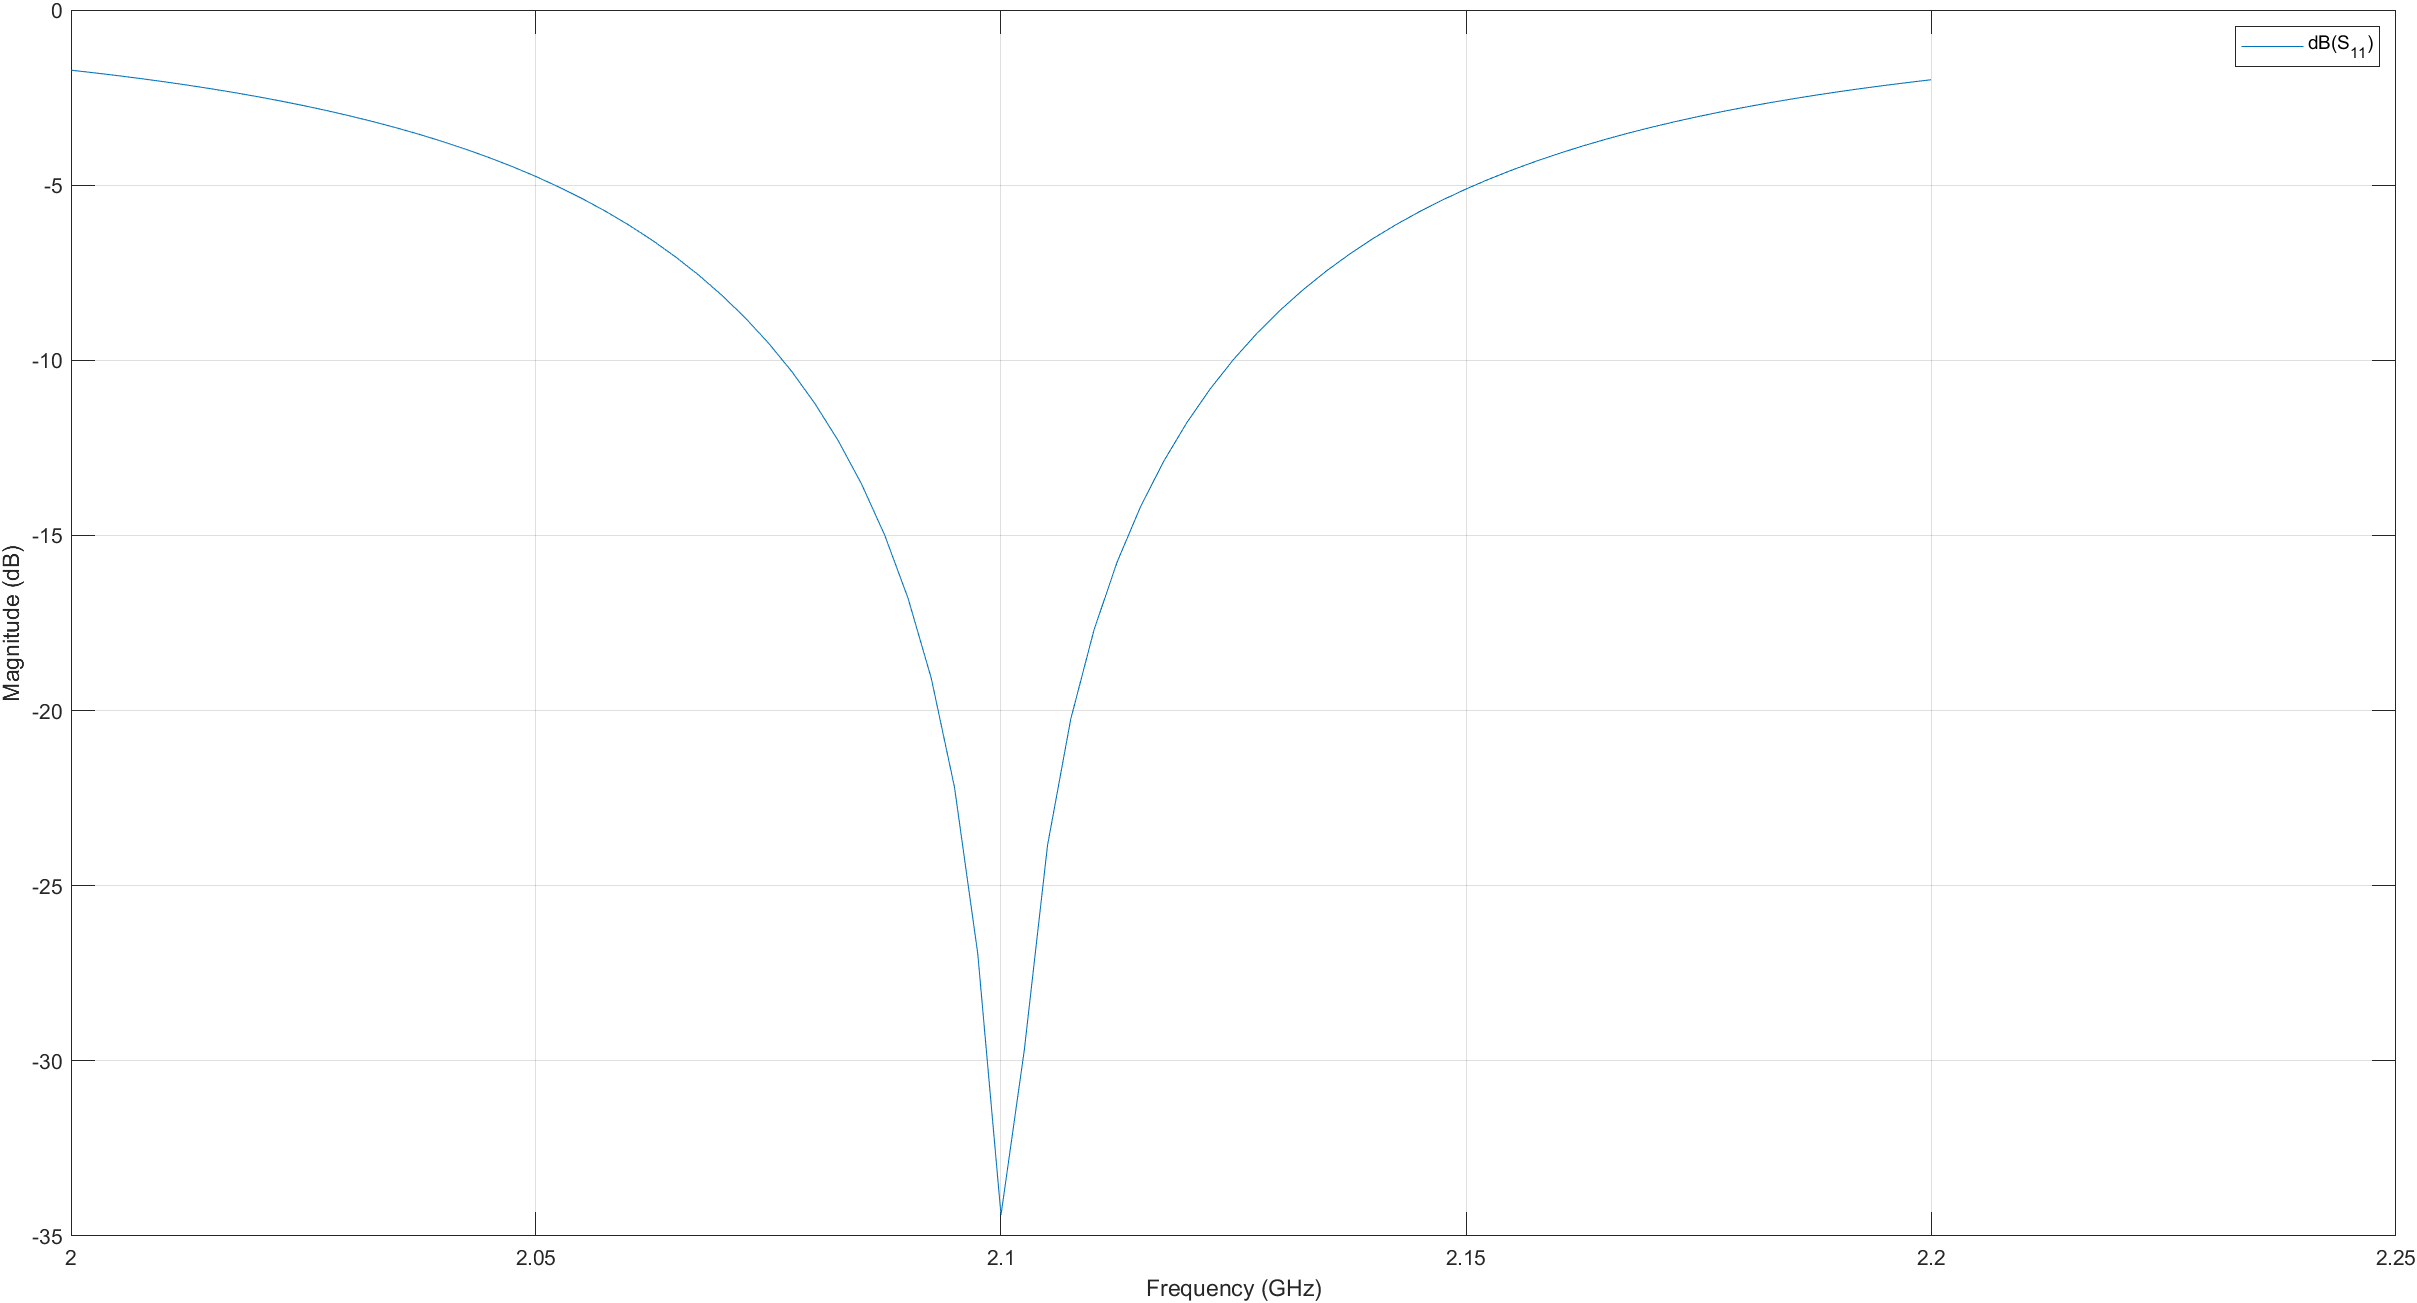
\includegraphics[width = 0.5\linewidth]{gamma.png}
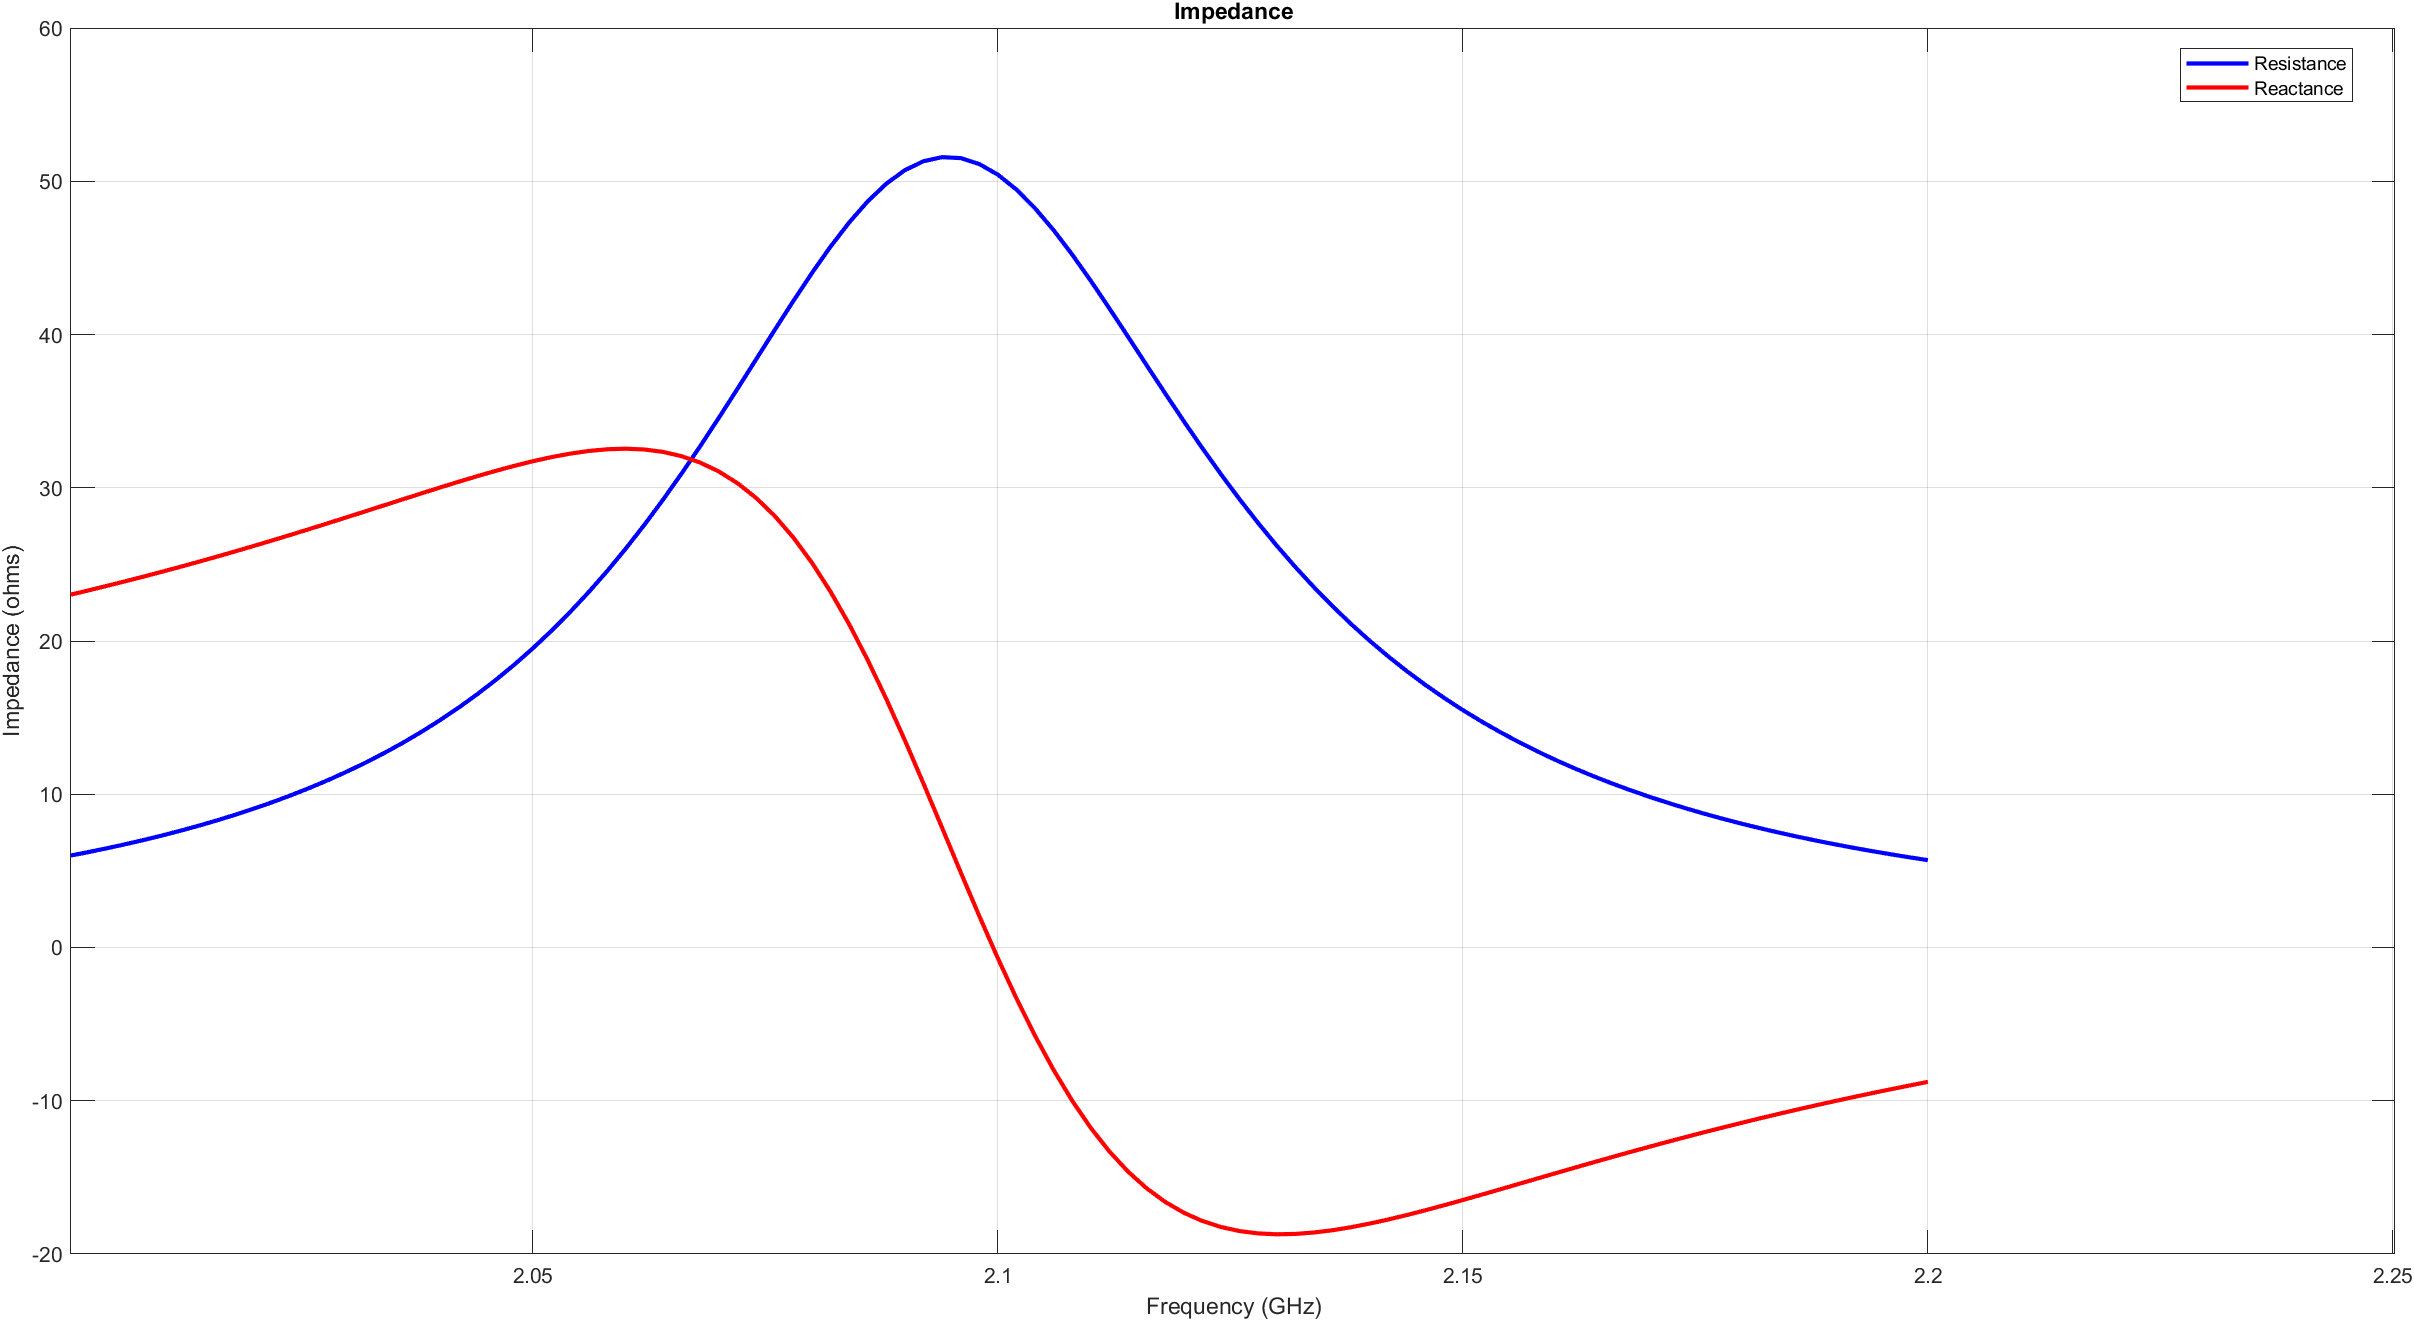
\includegraphics[width = 0.5\linewidth]{impedances.png}
\captionof{figure}{\color{gray}\fontfamily{lmss}\selectfont Reflection coefficient (left) and impedances (right) plots depending on $f\,\in\,2.0\div 2.1\,GHz$}
\end{figure}
\end{center}
\subsection*{\fontfamily{qag}\selectfont\color{Turquoise}Overall array performance evaluation}

















}
\end{document}